%% LyX 1.4.3 created this file.  For more info, see http://www.lyx.org/.
%% Do not edit unless you really know what you are doing.
\documentclass[11pt,english]{article}
\usepackage[T1]{fontenc}
\usepackage{geometry}
\geometry{verbose,a4paper,tmargin=2cm,bmargin=2cm,lmargin=1cm,rmargin=1cm,headheight=1cm,headsep=1cm,footskip=1cm}
\usepackage{float}
\usepackage{graphicx}

\makeatletter

%%%%%%%%%%%%%%%%%%%%%%%%%%%%%% LyX specific LaTeX commands.
%% Because html converters don't know tabularnewline
\providecommand{\tabularnewline}{\\}
\floatstyle{ruled}
\newfloat{algorithm}{tbp}{loa}
\floatname{algorithm}{Algorithm}

%%%%%%%%%%%%%%%%%%%%%%%%%%%%%% User specified LaTeX commands.
%% LyX 1.5.3 created this file.  For more info, see http://www.lyx.org/.
%% Do not edit unless you really know what you are doing.



\makeatletter

\makeatother

\AtBeginDocument{
  \def\labelitemiii{\(\bullet\)}
}

\usepackage{babel}
\makeatother
\begin{document}

\title{{\Large Specification and Implementation of a Python to SAGA Language
Binding}{\normalsize }\\
 {\normalsize Computer Science Master Thesis} {\Large }}


\author{P.F.A. van Zoolingen{\normalsize }\\
 {\normalsize 1284657, pzn400@few.vu.nl}}

\maketitle
\begin{abstract}
This thesis describes how we created a Python language binding for
SAGA, the Simple API for Grid Applications, and how we implemented
the language binding on top of the Java reference implementation.
Using this functionality, Python programmers can use SAGA to program
grid aware applications and shield themselves from all the details
which come with grids. The language binding and its implementation
add to the adoption of SAGA in a world of with many different APIs
and middleware layers.
\end{abstract}

\section{Introduction}

This section contains the introduction to this thesis. It is written
in both English and Dutch.


\subsection{Introduction English}

SAGA stands for Simple API for Grid Applications, and was developed
to offer users a simple tool to program applications for heterogeneous
grids. These grids often consist of different types of hardware, operating
systems and middleware software and are hard to program. SAGA is developed
to be independent of any underlying hardware or software and it shields
the user from all the details, and lets him focus on programming grid
aware applications.

To use the SAGA API, the functionality described by SAGA has to be
implemented by another piece of software: the SAGA implementation.
Currently, there are two different reference implementations which
are programmed in the programming languages Java and C++. In a general
sense, only Java and C++ applications can use the SAGA implementations
to access the grid in an easy way. This thesis describes how we added
another language to that list, namely Python. Python is partially
supported by the C++ reference implementation, but there is no specific
Python language binding available. A language binding is a set of
classes and methods which describes the SAGA functionality in a Python
specific way, independent of the chosen reference implementation.
During the course of my master project we have specified the Python
language binding and implemented the language binding for the Java
reference implementation.

This thesis is divided into different pieces. First we will describe
and explain what SAGA is, where it comes from and how it is implemented.
Then we will continue with a description of Python and a special implementation
of Python called Jython, followed by the specification of the language
binding and its implementation. After that we will describe the testing
processes of the language binding, the discussion of the project,
the future work and we will conclude with the conclusion.


\subsection{Introduction Dutch}

SAGA staat voor Simpele API voor Grid Applicaties en is ontwikkeld
als een simpel stuk gereedschap om het programmeren op heterogene
grids te vergemakkelijken. Dit soort grids bestaan vaak uit verschillende
hardware, besturingssystemen en middleware software en het is vaak
lastig om hier grid applicaties voor te programmeren. SAGA is ontwikkeld
als een aanspreekpunt voor het grid, onafhankelijk van de onderliggende
hard- en software. Tevens houdt de API de programmeur weg bij de onderliggende
details, die per platform zeer kunnen verschillen. De programmeur
kan zich hierdoor bezighouden met het programmeren van een hogere
abstractie niveau voor zijn applicatie.

Om de API te kunnen gebruiken moet de functionaliteit beschreven door
SAGA ge\"implementeerd worden door andere software, ook wel de SAGA
implementatie genoemd. Momenteel bestaan twee verschillende referentie
implementaties die gemaakt zijn in de programmeertalen Java en C++.
Dit houdt globaal in dat het alleen in de talen C++ en Java mogelijk
is om een applicatie te programmeren die door middel van SAGA het
grid te gebruikt. Deze master thesis beschrijft hoe daar een derde
taal aan toe is gevoegd, namelijk Python. Python word op dit moment
al deels ondersteund door de C++ referentie implementatie, maar er
is nog geen Python 'language binding' gespecificeerd die de syntax
voor Python applicaties vastlegt. De language binding specificeerd
een set van klassen en methodes die de SAGA functionaliteit beschrijft
in een Python specifieke manier, onafhankelijk van de onderliggende
referentie implementatie. Tijdens mijn master project heb ik een Python
language binding voor SAGA gespecificeerd en ge\"implementeerd bovenop
de Java referentie implementatie. Deze implementatie zou in theorie
moeten werken op elke Java implementatie van SAGA. 

Deze thesis is onderverdeeld in verschillende delen. Eerst zal ik
uitleggen wat SAGA is, waar het vandaan komt en hoe het ge\"implementeerd
is. Ik zal doorgaan met een beschrijving van Python en een specifieke
implementatie van Python genaamd Jython, gevolgd door de specificatie
van de language binding en zijn implementatie. Daarna zal ik het testen
van de language binding bespreken, de discussie van het project, het
mogelijke vervolg onderzoek na dit project en besluiten met de conclusie.


\section{SAGA}

In this section we will describe what SAGA is, how it was created
and the packages it consists of. In the last part we will discuss
the Java and C++ reference implementations and how they work.


\subsection{Short History of SAGA}

SAGA stands for Simple API for Grid Applications. SAGA came as an
idea in a time when multiple middleware projects and applications
groups were looking for higher-level programming abstractions and
the simplification of programming for the grid \cite{SAGA}. A SAGA
research group (SAGA-RG) was founded within the Global Grid Forum
(GGF), which later merged into the Open Grid Forum (OGF). The aim
of the group has been to identify a set of basic grid operations and
derive a simple consistent API, which eases the development of applications
that make use of grid technologies. 

To poll the needs of users, the research group sent out a call for
use cases. In these use cases users described many subjects such as
their application area, the desired look and feel of the API, and
resource, performance and security considerations. The majority of
use cases which were returned came from scientific users \cite{UseCases},
which probably biased SAGA in the analysis of the use cases towards
scientific applications. In this analysis, the research group focused
on the identification of the SAGA API scope, on the level of abstraction
wanted and needed by the application programmers. Non-functional requirements
and requirements from other projects, such as GAT \cite{GAT} and
CoG \cite{CoG} were also considered.

With 24 use cases available, the requirements from the users could
be distilled \cite{ReqAnalysis}. A design team was formed to use
these requirements to design and develop the API. A few general design
issues were considered and agree upon.

\begin{itemize}
\item The API would be designed and developed in a object-oriented manner
using a language-neutral representation.
\item Grid subsystems should be specified independent from each other to
allow independent development and implementation of parts of the API.
\item Sessions and security should be an essential part of SAGA since applications
often run across administrative domains and security boundaries.
\item Data management, like remote file access and replica catalogs are
an important part of grid applications and should therefore be part
of SAGA.
\item Remote jobs and asynchronous operations are a common requirement for
grid applications and must be supported in the API.
\item Asynchronicity is preferred to be handled by a polling mechanism rather
than a subscribe/listen mechanism to make implementations in non multi-threaded
environment easier.
\item SAGA should support inter-process communication as a stream concept,
similar to BSD sockets.
\end{itemize}
Ultimately, the purpose of SAGA is to provide an simple API that can
be used with much less effort compared to the vanilla interfaces of
existing grid middleware. A guiding principle for achieving this simplicity
is the 80/20 rule: serve 80\% of the use cases with 20\% of the effort
needed for serving 100 \% of all possible requirements and to provide
a standardized, common interface across various grid middleware systems
and their versions. 

After determining the requirements, a so-called SAGA Strawman API
was developed to accommodate the requirements and after some iterations
the SAGA API was published in January 2008 \cite{GFD.90}. SAGA is
described in a document called \emph{{}``A Simple API for Grid Applications
(SAGA)''} or GFD.90. GFD.90 specifies the core components of SAGA.
It has formed the basis of specification of the Python language binding,
which will be explained in section \ref{sec:Specification}, and the
reference implementations. It is aimed at implementors of the API
and not directly at end users. The implementors of the reference implementations
can supply the end users with the documentation and specific language
bindings.




\subsection{SAGA API }

SAGA is divided into two parts. The first part is the Look \& Feel
part which contains the base classes and interfaces. The second part
is the API part which represents explicit entities and actions of
some backend system.


\subsubsection{Look \& Feel}

The SAGA Look \& Feel is defined by a number of classes and interfaces
which ensure the non-functional properties of the SAGA API. Non-functional
requirements are requirements that specify criteria that can be used
to judge the operation of a system, rather than specific behaviors.

The interfaces and classes from the Look \& Feel are intended to be
used by the functional SAGA API packages

\begin{description}
\item [{Error}] The Error package contains all the exceptions which can
raised or thrown by SAGA API calls. GFD.90 also describes an \texttt{error\_handler}
which allows a user of the API to query for the latest error associated
with a SAGA object. Error handlers should not be included in language
bindings of languages which have exception handling capabilities of
their own, such as Python.
\item [{Object}] The \texttt{Object} package provides mechanisms which
are needed by all SAGA objects, such as cloning and getting the type,
ID and Session of the object. The \texttt{Object} class is also called
the \emph{base object}
\item [{URL}] The \texttt{URL} object is used to reference local and remote
resources. Using a separate \texttt{URL} object simplifies the construction,
parsing and checking of URLs in applications and unifies the signatures
of SAGA method calls that accept URLs.
\item [{Buffer}] SAGA has a generic buffer object that is designed as a
container for data. \texttt{Buffer} is used in combination with a
number of SAGA calls that perform byte-level I/O operations. The data
can be either allocated and maintained in application memory or be
managed by the SAGA implementation.
\item [{Session}] The Session object provides the functionality to interactively
exchange information between two computers and isolates independent
sets of SAGA objects from each other. Sessions support the management
of security information by using contexts.
\item [{Context}] The \texttt{Context} class is a container for security
information and is attached to a \texttt{Session} object to make the
information available to all objects instantiated in that session.
Multiple contexts can co-exist in one session for different method
calls and can be shared between sessions. 
\item [{Permission}] The \texttt{permission} package contains an interface
to let applications allow or deny specific operations on SAGA objects
or grid entities for different types of users. Because it is difficult
to anticipate how different types of middleware handle these permissions,
applications using the \texttt{permission} package are not expected
to be fully portable between SAGA applications. In addition, each
implementation must specify which permissions it supports and for
which operations.
\item [{Attributes}] The \texttt{attributes} package provides an interface
for storing and retrieving attributes associated with SAGA objects.
The supported attributes of an object are included in the description
of the object in the language binding. 
\item [{Monitoring}] The \texttt{monitoring} package provides a mechanism
to monitor certain properties of monitorable SAGA objects by exposing
metrics to the application. These metrics which represent monitorable
entities, such as state or CPU time used. Steerable objects even allow
certain metric values to be changed. An example of a monitorable object
is a \texttt{Task.} The \texttt{Task} object has a \texttt{task.state}
metric which can be monitored. If a special object, called a \texttt{Callback},
is attached to the task and the state changes, the SAGA implementation
calls the \texttt{cb()} method of the \texttt{Callback} to respond
to the state change of the task.
\item [{Task}] The last package of the look \& feel is \texttt{task}. Tasks
are representations of asynchronous operations and each SAGA object
that implements the \texttt{async} interface is obliged to offer synchronous
and asynchronous method calls. 
\end{description}

\subsubsection{API Packages}

The interfaces, classes and methods defined in the API or functional
packages of GFD.90 are, in general, representing explicit entities
and actions of some backend system. The currently specified packages
are shown below, but new packages may be added in the future.

\begin{description}
\item [{Job}] The \texttt{job} package offers the functionality to submit
jobs to grid resources and to monitor and control these jobs. Job
submission can be done in batch mode or interactive mode. Jobs be
controlled through different methods calls such as \texttt{run()}
and \texttt{suspend()}. Status information can be retrieved for both
running and completed jobs. 
\item [{Namespace}] The \texttt{namespace} package describes notions of
hierarchical namespace entries and directories. These \texttt{NSEntry}
and \texttt{NSDirectory} objects allow to navigate through a namespace
such as filesystems. Operations like moving, renaming, copying or
removing these namespace entries are also supported.
\item [{File}] The \texttt{file} package is an extension of the \texttt{namespace}
package and, in addition to all the operations from \texttt{namespace},
allows access to the contents of the files regardless of their location.
It also offers the Scattered, Pattern-Based and Extended I/O paradigms.
\item [{Replica}] The \texttt{replica} package describes the interaction
with replica systems, especially logical files, logical directories
and creating replicas. A logical file is a namespace entry with some
metadata and associated set of physical replica files. A replica (or
physical file) is a file which is registered on a logical file. In
general, all replicas registered on the same logical file are identical,
but can be on different machines in the grid. 
\item [{Stream}] The \texttt{stream} package specifies the functionality
to create simple remote socket to establish connections between components.
These components can then form a distributed application together.
\item [{RPC}] The Remote Procedure Call (RPC) or \texttt{rpc} package specifies
operations to execute code on other machines. This is done by invoking
methods on different machines. A high level API called GridRPC \cite{GridRPC}
is imported into SAGA and adapted to the SAGA look and feel. Semantically,
GridRPC maps to the RPC package.
\end{description}

\subsection{Reference Implementations}

SAGA currently has two reference implementations, one written in Java
and one written in C++. In this section we will explain what they
are and how they work.


\subsubsection{Java SAGA Reference Implementation}

After GFD.90 was released in January 2008, a Java SAGA reference implementation
was created at the Vrije Universiteit and released in September 2008
\cite{SJava}. It is largely based on JavaGAT \cite{JavaGAT}, a toolkit
which provides a high-level middleware-independent and site-dependent
interface to grids. JavaGAT is the reference implementation for the
GAT API \cite{GAT}, which shares many goals with SAGA. Common goals
are the aim to make it easier for grid users to create complex grid
applications and to shield them from the underlying middleware. 

The structure of JavaGAT can be seen in figure \ref{fig:JavaGAT structure}.

\noindent \begin{center}\texttt{}%
\begin{figure*}
\begin{centering}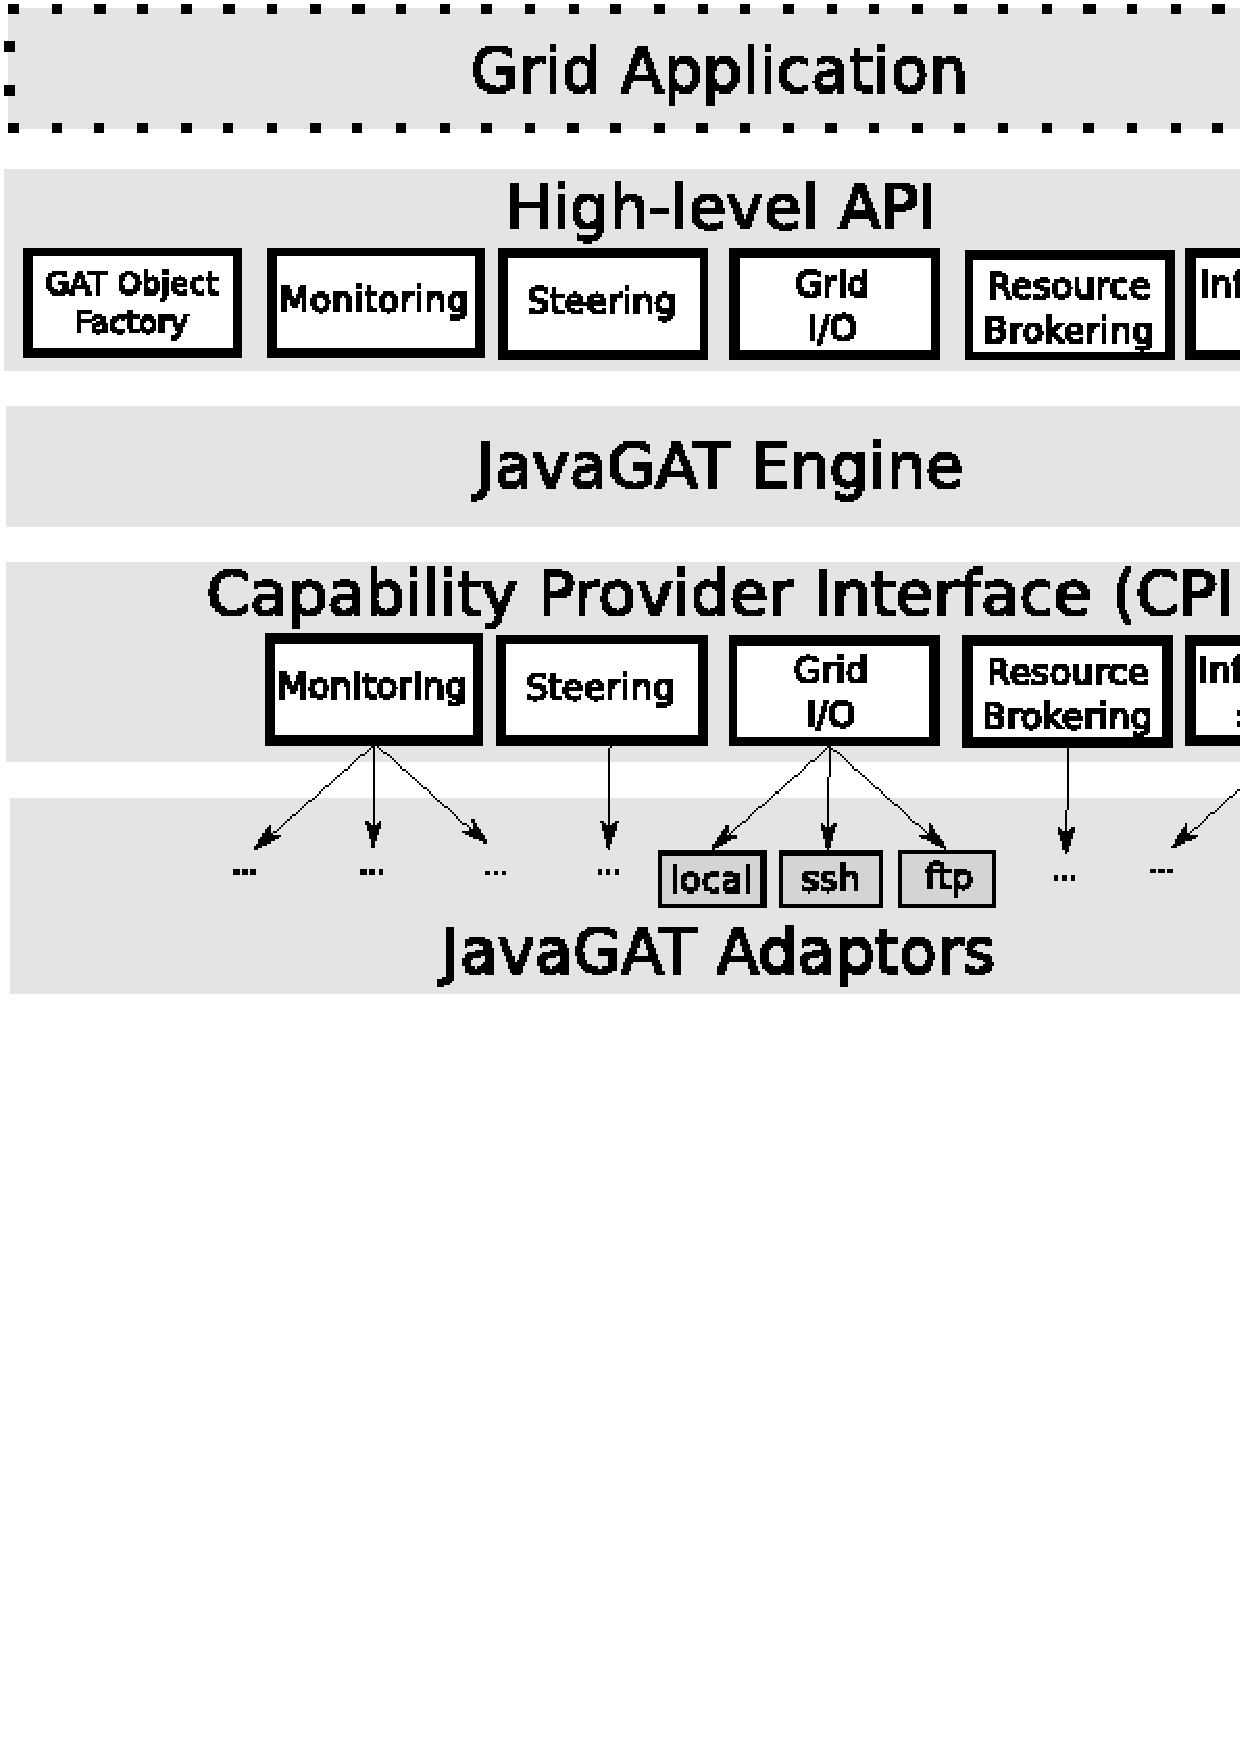
\includegraphics[bb=0bp 365bp 694bp 842bp,scale=0.5]{JavaGATFigure}\par\end{centering}


\caption{\label{fig:JavaGAT structure}The structure of the JavaGAT implementation,
taken from \cite{JavaGAT}}
\end{figure*}
\par\end{center}

The Java SAGA reference implementation consists of different layers
which all have its own responsibility. The top layer is the API that
serves as the interface to the user. Below the API resides the engine.
The engine is responsible for delegating the API calls to the correct
middleware. The Capability Provider Interface is the layer which connects
the engine to middleware specific software, called \emph{adaptors}.
When the engine receives a request, e.g., to copy a file, it selects
the right adaptor with help from the CPI. The adaptor then delegates
the copy request to the actual middleware that copies the file. 

Principles used from JavaGAT in the SAGA Java reference implementation
include intelligent dispatching, nested exceptions and the adaptor
writing framework. Intelligent dispatching is the process where the
engine chooses the correct adaptor for the requested action and the
related preferences {[}ADD MORE INFO]. Nested exceptions are special
aggregations of exceptions which come from the different adaptors.
Adaptors might raise exceptions when they fail at a certain action
or do not implement the requested action. All these exceptions are
stored in a nested exception which is only thrown to the grid application
after every adaptor failed at fulfilling the request. The adaptor
writing framework makes it easy for users to write or change adaptors
with little effort. This is an advantage because there are many middleware
systems available and they are changing often.

The Java reference implementation implements SAGA completely since
this is a requirement in the SAGA specification to be called fully
compliant. Implementation which do not implement all specified methods
are called partially compliant. There are still some deviations from
GFD.90, such as symbolic links and permissions. Java does not have
a notion of symbolic links and permissions so it is not possible to
include them. If methods relating to them are called, the implementation
will throw a \texttt{NotImplementedException}. The implemented Java
language binding also contains small extensions like file streams
and using RPC with objects instead of using byte arrays.

Adaptors currently included with the Java reference implementation
are XMLRPC for RPC, Socket for streams, Gridsam for jobs, and Adaptors
from JavaGAT {[}ADD MORE INFO ON ADAPTORS].


\subsubsection{C++ SAGA Reference Implementation}

Before the GFD.90 specification for SAGA was released, a group at
the Louisiana State University \cite{LSU} started to build a C++
reference implementation \cite{C++SAGA}. People from that group were
also involved in the SAGA design process and the development of GAT,
and pioneered in implementing a SAGA C++ implementation. This implementation
works in a similar way as the Java implementation. It also includes
call routing through to the adaptors, the probing of multiple adaptors
and the variable adaptor strategies. In addition, it tries latency
hiding strategies such as bulk optimization and automatic load distribution
over multiple adaptors.

The C++ reference implementation offers wrappers for C and Python,
but they are in alpha stage and therefore not fully functional. A
Python language binding is not available and the wrapper closely follows
the syntax of the underlying C++ layer. The Python language binding
described in this thesis is specified top-down from the SAGA specification,
the wrapper is designed bottom-up from the implementation {[}ADD WHAT
IS BETTER].


\section{Python}

The Python language binding for SAGA is a specification of the classes
and methods in the programming language Python. In this section we
will explain parts of Python and how it influences the specification. 


\subsection{Introduction to Python}

Python was created in 1989 by Guido van Rossum who was working at
the Centrum voor Wiskunde en Informatica (CWI) in the Netherlands.
He worked on the programming language ABC, but needed some extra features.
Not wanting to fall back to C, he created his own language called
Python. 

Python is a high level interpreted scripting language and applications
do not have to be explicitly compiled. It is Object Oriented but also
borrows some features from functional languages. The Python interpreter
is written in C, sometimes called CPython, and is extensible by writing
your own modules or by writing special C modules for it. Because the
interpreter is written in C it is portable to platforms which support
the ANSI C compiler and scripts have to be written only once to be
run on many platforms. Some projects have rewritten the interpreter
in different programming languages to take advantage of the distinct
features of the language. These projects include Jython for a Java
interpreter and IronPython for a C\# version. According to estimations
\cite{ProgLang}, the popularity of Python is around 5\%, after Java,
C, C++, VB and PHP. This rating is based on information from search
engines, engineers and companies world-wide. Together with Java, C++
and C, support for Python will give users enough choice for developing
applications using SAGA.


\subsection{Syntax Features}

Python has some features in its syntax which influenced the SAGA language
binding, and makes one to one copying of the SAGA specification not
as straight forward as it seems. In this section we will explain which
features those are.


\subsubsection{Dynamic Typing}

Python uses dynamic typing, which means that the type of a variable
is bound to the type of variable value, and can change regularly.
In static typing, the type is set when the variable is created and
cannot be changed afterwards. This gives new possibilities when dealing
with return values and parameter types. A commonly heard term is that
Python uses 'Duck Typing' ({}``If it looks like a duck and quacks
like a duck, it must be a duck.\char`\"{}). This means that calling
a method of an object is always possible. If it actually succeeds
and does not result in a runtime error depends on the object. In this
context it means that if you can call quack() and walk() on an object,
the type was probably Duck. If it gave a runtime error, the object
was definitely not a Duck. There are ways check the type of a variable,
like \texttt{type(), isinstance(), issubclass() or variable.\_\_class\_\_}
.


\subsubsection{Keywords and built-ins}

\label{sub:Keywords-and-builtins}Python has reserved keywords just
like every programming language. Most of these are are similar to
other languages, but Python has some specific ones which are also
used in the SAGA specification. In the \texttt{Permission} enum \texttt{Exec}
and \texttt{None} are mentioned, but both \texttt{exec} and \texttt{None}
are reserved. Although Python is case-sensitive, this gives problems
when defining a consequent naming scheme.

Python also has some standard functions which are available. These
include functions like \texttt{list()}, \texttt{tuple()}, \texttt{dir()}
and \texttt{type()}. SAGA has some parameters names like which interfere
with the built in methods, such as \texttt{type} in the \texttt{Metric}
constructor.


\subsubsection{Methods}

Methods are defined in Python by using the \texttt{def} keyword followed
by the method name and the parameters in brackets. \texttt{def} defines
a method, but can also be used to overwrite the previously defined
method with the same name. This makes it impossible to do overloading,
defined as defining multiple methods with the same name but only differing
in parameter types. The same effect can still be achieved in Python
since the parameter type is not defined in the method declaration.
It does give difficulties if SAGA specification has overloaded methods
with completely different sets of parameter types.


\subsubsection*{Multiple Return Values}

Python also supports returning multiple variables from one method
call opposed to many other languages. This prevents using special
objects which hold more variables or special global variables. The
actual returned type is a special read-only list called a tuple, but
users can use multiple variables to automatically unpack the tuple
among the variables. See algorithm \ref{alg: multi ret values} for
an example.

%
\begin{algorithm}[h]
\texttt{def method():}

\texttt{~~~~variable1 = 'a String'}

\texttt{~~~~variable2 = 2}

\texttt{~~~~return variable1, variable2}~\\
 \texttt{}

\texttt{var1, var2 = method()}


\caption{\label{alg: multi ret values}Example of multiple return values in
Python}
\end{algorithm}


Since the variables are dynamically typed, the same method can return
multiple variables of different types. This feature is usable with
the \texttt{JobService.run\_job()} method since that method is specified
to return the job and three handles to the standard input, output
and error.


\subsubsection*{Default Parameter Values}

In the method declaration it is possible to specify default values
for parameters in the method definition. Not all parameters need default
values, but those that do specify them, need to be placed at the end.
Python needs this order to determine which given value in the method
call belongs to which parameter. See algorithm \ref{alg:Expl-defparameters}
for an example.

%
\begin{algorithm}[h]
\texttt{def write( buffer, size=3, offset=5):}

\texttt{~~~~pass}~\\


\texttt{write( buf )}

\texttt{write( buf, 3 )}

\texttt{write( buf, 3, 5 )}

\texttt{write( buf, offset=5 )}

\texttt{write( offset=5, size=3, buffer=buf)}


\caption{\label{alg:Expl-defparameters}Example of default parameters in Python.
Each \texttt{write()} call has exactly the same parameter values.
The \texttt{pass} statement does nothing, but leaving the method empty
will result in a syntax error. Python uses whitespace to define blocks
of code, also called suites.}
\end{algorithm}



\subsubsection*{Named Parameters}

When looking at the example of algorithm \ref{alg:Expl-defparameters}
you can notice that in the last two writes the parameter names are
explicitly mentioned. This explicit naming of the parameters allows
that when dealing with a large amount of defaulted parameters, you
can specify which parameters you want to change in the method call
instead of specifying all the parameters. An example is shown in algorithm
\ref{alg:Example-of-explicitly}.

%
\begin{algorithm}[h]
\texttt{def method( first=1, second=2, third=3, last = '4'):}

\texttt{~~~~pass}~\\


\texttt{method ( last = 'final')}


\caption{\label{alg:Example-of-explicitly}Example of explicitly naming the
parameters}
\end{algorithm}


To improve usability in the Python language binding, deciding about
the order of the defaulted parameters is an interesting issue. A \texttt{File.read()}
call from the SAGA specification defined as \texttt{read(size='-1',
buffer=None)} has a different parameter order than a \texttt{File.write()}
call which is defined as \texttt{write( buffer, size='-1').} This
looks inconsistent, but is done because a data buffer is needed for
writing, but is optional for reading. The read data is returned as
a string. The amount of data read can be checked by doing a \texttt{len()}
call with the string as parameter, i.e: \texttt{len(returnedString)} 


\subsubsection*{Different Data Types}

Although Python supports many data types, it misses some types which
are standard in other languages and are mentioned in GFD.90. These
include enum, byte and char. Characters are just strings with a length
of one. The array package does have notion of a character to store
strings of length one, but there is no separate data type.

Python has no notion of an enum, but this can be solved in different
ways. First of all, a class can be constructed containing all the
values from the enum, such as the Flag enums in the SAGA specification.
Another solution is to use dictionaries, which have similarities with
hashtables in other languages. Dictionaries are commonly used in Python,
but their syntax is less straightforward than using simple objects
filled with variables.

The byte data type is missing from Python. This causes some confusion
how to specify and implement the mutable Buffer defined in SAGA. The
Buffer encapsulates a sequence of bytes to use in read and write operations
and is an essential part of SAGA. A possibility is to deny users to
use application managed buffers and use implementation managed buffers
only, but this would limit the use of Buffers in SAGA and exclude
a part of SAGA from the language binding. There is no standard to
use buffers and they are not available in Python. Users could write
their own buffer library, but it defeats the platform independent
principle. 

A solution was found in using arrays of chars. Arrays are guaranteed
to contain only the specified data type and if characters are read
or written they are immediately visible to users. Problems may arise
if underlying implementations use different encodings for the characters,
like Unicode, but that should be solved the programmers implementing
the language binding. Suggestions were made to me to completely remove
the buffers since they would be not \emph{Pythonesque} or \emph{Pythonic}%
\footnote{Although \emph{Pythonic} is an extremely vague term, Python programmers
generally assume there is only one correct way to do something. Other
solutions are not \emph{Pythonic}.%
}.

Python also has support for numbers. Normally programmers will only
need an int. Int is internally implemented as a C long. If the int
overflows because two very large numbers are multiplied, Python will
automatically switch to a long. Longs can be arbitrarily long. Python
has no double but only a double-precision float. Shorts are not available
in Python.


\subsubsection{Extending Python}

As mentioned earlier, it is possible to write libraries for Python
and import them dynamically. These libraries can be written in Python
but it is also possible to write them in C or C++. Using predefined
data types and structs it is possible to program a library which is
usable by the CPython interpreter. This possibility can be used to
speedup performance in certain loops or to add functionality to applications
which is not available in standard Python. The downside of this mechanism
is that the switching between the library and the interpreter takes
some time and would mean a performance hit for simple calls which
could also be done in standard Python. The writing of these libraries
is not trivial and uses many Python specific data types and syntax.
Fortunately there are tools available which help in this task such
as SWIG \cite{SWIG} and Boost \cite{boost.python}. The Boost.Python
library is used in the C++ reference implementation to create their
Python wrapper, and thus making the SAGA functionality available to
Python users.

During the specification of the Python language binding we have used
the features which are already available in the language and have
avoided using features which would mean that extra libraries would
have be added. It was planned that the specification could be implemented
by using the standard Python distribution or derivatives like Jython.


\subsubsection{\label{sub:Version-of-Python}Version of Python}

The language binding consists mostly out of class and method declarations
and conforms to the current 2.6 version of Python which was released
in October 2008. Although this does not say much about underlying
implementations of the language binding, these declarations are not
expected to change or become invalid in upcoming versions of Python.
In December 2008, version 3.0 was released. It is stated that this
version is incompatible with the previous versions. 

There are some changes which effect the language binding. Version
3.0 implements a byte data type \cite{bytePEP},\cite{PyLibFunctions}
and a mutable byte buffer\cite{byteByfferPEP} as a byte array. These
changes will severely simplify the specification and implementation
of the \texttt{Buffer} class and the \texttt{Iovec} class. These classes
now work with char arrays to emulate bytes. The Parameter class from
the rpc package will also be helped with introduction of a byte data
type because it simplifies the use of method calls which require byte
arrays or byte buffers. There is also a proposal for overloading and
interfaces \cite{overloadingPEP} . Interfaces would be defined as
classes having abstract methods without an implementation. These interfaces
would be more suitable to implement the interfaces defined in GFD.90.
Abstract base classes \cite{abstractBaseClasses} are supported since
version 2.6 roughly do the same. These 'Python Enhancement Proposals'
or PEPs would solve difficulties that were raised in the 2.x versions
of Python. Now that Python 3.0 is released, it will take some time
before it is excepted as the mainstream version for Python programmers.
In addition to that, it will take some time before the other implementations
like Jython will fully support version 3.0.


\subsection{Jython}

Python is not the only interpreter of Python source code as there
are multiple implementations available at this point. Stackless \cite{stackless}
has all the functions of the reference implementations but does not
use an internal stack which makes it useful for multi-threaded Python
applications. The implementation in .Net is called IronPython \cite{ironpython}
and the implementation in Java is called Jython \cite{jython}. These
implementations allow users to make use of Python and Java or .Net,
which adds possible solutions for solving a problem. They can take
advantage of features from both languages and all tools and libraries
which are written in them.

This is where SAGA comes in. To use let a Python application use the
C++ implementation, it can access it through the wrapper. To let it
access the Java implementation we have to use something different
than the Python reference implementation. The solution for this is
to run Python applications on the Jython interpreter which can use
the underlying SAGA implementation.

Jython was first called JPython when it was created in late 1997 by
Jim Hugunin. In 2000 it was moved to SourceForge and renamed to Jython.
Its current version is 2.2.1 with the 2.5 release coming around January
2009. This 2.5 release will probably have the same features as the
2.5 release of the Python reference implementation. 


\subsection{Differences between Jython and Python}

Jython and Python are actually the same language, but there are some
differences between them. An out-dated list of them can be found at
\cite{diffJyPy}, which shows that differences are mostly in behavior
between the two interpreters. Jython also lacks some built-in modules
and modules like Numeric for scientific calculations. It will always
lag behind the reference implementation since new features and changes
to the language are designed and implemented there first. The Java
language also misses features which deal with operating system specific
issues such as links and permissions.

When taking all the differences into account, it should be possible
to create applications which run on both the CPython and the Jython
interpreter as long the programmer remembers to keep the differences
into account.


\section{Specification\label{sec:Specification}}

This section describes how the specification of the Python language
binding was designed and what choices were made in the process. Although
the complete specification, including all the notes of the 16 modules,
55 classes and more than 200 methods, would be to much to be included
within this thesis, we will describe most design decisions.


\subsection{Global Design Decisions}

The specification for the language binding was inspired by three things;
The GFD.90 \cite{GFD.90} document, the Python style guide \cite{styleGuide}
and suggestions given on the saga-rg mailinglist. Since we did not
have much experience with Python the people on the mailinglist gave
us quite some insight about proper syntax and programming constructs.
The style guide was a good start to set the rules on how the specification
should look like. GFD.90 contained all specifics on SAGA itself and
is the primary source of information related to SAGA. Most naming
was directly taken from the document, just as all the documentation.

The layout of the packages is simple. The root of the package structure
is \texttt{saga}. This is the name of a directory containing all the
modules. The modules are files with the \texttt{.py} extension and
contain the classes which are related to each other and are defined
as a package in the GFD.90 document. Python recognizes this structure
of a directory, module files and a special \texttt{\_\_init\_\_.py}
file as a complete package is able to import them. For example the
URL class can be imported with the statement \texttt{from saga.url
import URL}. 

All the document strings in the specification are complemented with
special statements used by an application called Epydoc \cite{epydoc}.
Epydoc can generate a browsable version of the language binding which
helps application programmers designing Python programs using SAGA.
Almost all documentation in the document strings comes from GFD.90
and is adapted to the language binding.

I have used the CapitalizedWords convention for the naming of classes,
the all-lowercase convention for package and module names, the all-lowercase
with underscores for the method names, the parameter names and variable
names, and the UPPERCASE convention for constants. These conventions
come from the style guide with the exception of convention for constants.
Using all-lowercase or CapWords would create clashes between some
constants and reserved keywords as mentioned in section \ref{sub:Keywords-and-builtins}.

Interfaces do not exist in Python, but GFD.90 does define them. Interfaces
are specified as normal classes, with the specified methods in them.
Implementations of the language binding should make sure that instantiating
an 'interface' class does not work since it makes no sense to do so. 

Since enumerations do not exist in Python but GFD.90 does define them,
we have specified the enums as normal classes in the specification.
These classes contain the constants from the enums. 

I have mapped the possible return types to their Python counterpart,
such as strings to strings, numbers to ints and arrays to lists.

To deal with asynchronous methods and the task creation we have added
a tasktype parameter to all methods in classes which are subclasses
of the Async class. This parameter is the last one of all the defined
parameters and defaulted to \texttt{TaskType.NORMAL}. This means that
by default the method is executed synchronous and returns its specified
return value and not a \texttt{Task} object. By placing the parameter
last and by defaulting it, it the syntax of the synchronous and asynchronous
calls stay consistent and should not interfere with each other.

Get and set methods are not regarded as \emph{Pythonic,} but GFD.90
requires them for the language binding to be fully compliant. Therefore
many class variables on which the getters and setters operate can
also be accessed through so-called properties. In the description
of the packages we shall mention the properties where they are defined.


\subsection{Error}

\begin{center}%
\begin{table}[h]
\begin{centering}\begin{tabular}{|l|l|}
\hline 
\texttt{None}&
\texttt{\_\_init\_\_(self, message, saga\_object=None) }\tabularnewline
&
Initialize an Exception object.\tabularnewline
\hline
\texttt{string}&
\texttt{get\_message() }\tabularnewline
&
Returns the message associated with the exception.\tabularnewline
\hline
\texttt{Object}&
\texttt{get\_object() }\tabularnewline
&
Returns the SAGA Object associated with the exception.\tabularnewline
\hline
\end{tabular}\par\end{centering}


\caption{\label{tab:ErrorMethods}Specified methods in Error module}
\end{table}
\par\end{center}

The \texttt{Error} module consists out of a \texttt{SagaException}
class which features the methods from table \ref{tab:ErrorMethods}
and 11 subclasses of the \texttt{SagaException} which are shown in
table \ref{tab:Subclasses-of-SagaException}. We have placed the \texttt{sagaObject}
parameter behind the message parameter because not all exceptions
contain an object and thus the \texttt{saga\_object} is optional.
\texttt{\_\_init\_\_} contains both constructors mentioned in GFD.90. 

\texttt{SagaException} exposes the properties \texttt{message} and
\texttt{saga\_object} to directly get the message and the associated
base \texttt{Object}.

\begin{center}%
\begin{table}[h]
\begin{centering}\begin{tabular}{|c|c|c|c|}
\hline 
\texttt{NotImplemented}&
\texttt{IncorrectURL}&
\texttt{BadParameter}&
\texttt{AlreadyExists}\tabularnewline
\hline 
\texttt{DoesNotExist}&
\texttt{IncorrectState}&
\texttt{PermissionDenied}&
\texttt{AuthorizationFailed}\tabularnewline
\hline 
\texttt{AuthenticationFailed}&
\texttt{Timeout}&
\texttt{NoSuccess}&
\tabularnewline
\hline
\end{tabular}\par\end{centering}


\caption{\label{tab:Subclasses-of-SagaException}Subclasses of SagaException}
\end{table}
\par\end{center}

Python has exception-handling capabilities and does not need the \texttt{error\_handler}
interface.


\subsection{Object}

The Object module contains the \texttt{ObjectType} class and the \texttt{Object}
class. \texttt{ObjectType} was originally designed as an enum but
is now a class with constants that are returned by objects to describe
their type. \texttt{Object} was an interface, but is now a class with
the same methods. The methods are shown in table \ref{tab:ObjectMethods},
and are not different from the GFD.90 specification. \texttt{get\_type()}
returns a value from \texttt{ObjectType} which happen to be integers
and \texttt{clone()} returns a deep copy of an object which is an
object itself.

\texttt{Object} exposes the properties \texttt{id} to get the object
ID, \texttt{type} to get the object type and \texttt{session} to get
the \texttt{Session} of the object.

\begin{center}%
\begin{table}[h]
\begin{centering}\begin{tabular}{|l|l|}
\hline 
\texttt{string}&
\texttt{get\_id(self)}\tabularnewline
&
Query the object ID.\tabularnewline
\hline 
 \texttt{int }&
\texttt{get\_type(self)}\tabularnewline
&
Query the object type.\tabularnewline
\hline 
\texttt{Session}&
\texttt{get\_session(self)}\tabularnewline
&
Query the objects session.\tabularnewline
\hline 
\texttt{Object}&
\texttt{clone(self)}\tabularnewline
&
Deep copy the object.\tabularnewline
\hline
\end{tabular} \par\end{centering}


\caption{\label{tab:ObjectMethods}Methods from the Object class}
\end{table}
\par\end{center}


\subsection{URL}

The \texttt{url} package contains only the \texttt{URL} class. The
methods defined in \texttt{URL}, shown in table \ref{tab:URLMethods},
are practically the same as defined in GFD.90. \texttt{URL} is a subclass
of \texttt{Object} and thus inherits all its methods and properties.
Additional properties exposed by \texttt{URL} are \texttt{string,
scheme, host, port, fragment, path, query} and \texttt{userinfo}.

\begin{center}%
\begin{table*}
\begin{centering}\begin{tabular}{|l|l|}
\hline 
&
\texttt{\_\_init\_\_(self, url='')}\tabularnewline
&
Initialize an URL instance.\tabularnewline
\hline 
&
\texttt{set\_string(self, url='')}\tabularnewline
&
Set a new url.\tabularnewline
\hline 
\texttt{string}&
\texttt{get\_string(self)}\tabularnewline
&
Retrieve the url as string.\tabularnewline
\hline 
&
\texttt{set\_scheme(self, scheme='')}\tabularnewline
&
Set the scheme of the url.\tabularnewline
\hline 
\texttt{string}&
\texttt{get\_scheme(self)}\tabularnewline
&
Get the scheme of the url.\tabularnewline
\hline 
&
\texttt{set\_host(self, host='')}\tabularnewline
&
Set the host of the url.\tabularnewline
\hline 
\texttt{string}&
\texttt{get\_host(self)}\tabularnewline
&
Get the host of the url.\tabularnewline
\hline 
&
\texttt{set\_port(self, port=-1)}\tabularnewline
&
Set the port of the url.\tabularnewline
\hline 
\texttt{int }&
\texttt{get\_port(self)}\tabularnewline
&
Get the port of the url.\tabularnewline
\hline 
&
\texttt{set\_fragment(self, fragment='')}\tabularnewline
&
Set the fragment of the url. \tabularnewline
\hline 
\texttt{string}&
\texttt{get\_fragment(self)}\tabularnewline
&
Get the fragment of the url.\tabularnewline
\hline 
&
set\_path(self, path='')\tabularnewline
&
Set the path of the url. \tabularnewline
\hline 
\texttt{string}&
\texttt{get\_path(self) }\tabularnewline
&
Get the path of the url.\tabularnewline
\hline 
&
\texttt{set\_query(self, query='')}\tabularnewline
&
Set the query of the url.\tabularnewline
\hline 
\texttt{string}&
\texttt{get\_query(self)}\tabularnewline
&
Get the query of the url.\tabularnewline
\hline 
&
\texttt{set\_userinfo(self, userinfo='')}\tabularnewline
&
Set the userinfo of the url. \tabularnewline
\hline 
\texttt{string}&
\texttt{get\_userinfo(self) }\tabularnewline
&
Get the userinfo of the url.\tabularnewline
\hline 
\texttt{URL}&
\texttt{translate(self, scheme)}\tabularnewline
&
Translate an URL to a new scheme.\tabularnewline
\hline
\end{tabular}                 \par\end{centering}


\caption{\label{tab:URLMethods}Methods from the URL class}
\end{table*}
\par\end{center}


\subsection{Buffer }

The buffer package contains only the Buffer class. Buffer contains
the methods shown in table \ref{tab:BufferMethods}.

\begin{center}%
\begin{table}[h]


\begin{centering}\begin{tabular}{|c|c|}
\hline 
&
\texttt{\_\_init\_\_(self, size=-1, data=None)}\tabularnewline
&
Initialize an I/O buffer.\tabularnewline
\hline 
&
\texttt{\_\_del\_\_(self) }\tabularnewline
&
Destroy a buffer.\tabularnewline
\hline 
&
\texttt{set\_size(self, size=-1) }\tabularnewline
&
Set size of buffer.\tabularnewline
\hline 
\texttt{int}&
\texttt{get\_size(self)}\tabularnewline
&
Retrieve the current value for size.\tabularnewline
\hline 
&
\texttt{set\_data(self, data, size=-1) }\tabularnewline
&
Set new buffer data.\tabularnewline
\hline 
\texttt{char array, list }&
\texttt{get\_data(self)}\tabularnewline
\texttt{or string}&
Retrieve the buffer data.\tabularnewline
\hline 
&
\texttt{close(self, timeout=-0.0)}\tabularnewline
&
Closes the object.\tabularnewline
\hline
\end{tabular}    \par\end{centering}


\caption{\label{tab:BufferMethods}Methods from the Buffer class}
\end{table}
\par\end{center}


\subsection{Session }


\subsection{Context }


\subsection{Permission }


\subsection{Attributes }


\subsection{Monitoring }


\subsection{Task }


\subsection{Job }


\subsection{Namespace }


\subsection{File }


\subsection{Replica }


\subsection{Stream }


\subsection{RPC }


\section{Implementation}

variable classes not write protected


\subsection{Previous work // Solutions Tested}


\subsection{Delegate Object}


\subsection{Convert Exception}


\subsection{Tasks}


\subsection{Inheritance}


\subsection{Get\_id()}


\subsection{All Modules Specified with Design Decisions}


\section{Testing}


\subsection{Test Environment}


\subsection{scripts}


\subsection{Bugs}


\subsection{Repository}


\section{Discussion}

This master project has delivered a Python language binding for SAGA
and an implementation for the language binding on top of the Java
SAGA reference implementation. Programmers can use the specification
of the language binding to use SAGA in their Python applications.
Our opinion is that the specification is user friendly and conforms
to how Python programmers would like to see the SAGA API. The specification
consists out of standard Python data types and looks like an easily
understandable API. 

The specification of the \texttt{Buffer}, \texttt{IOVec} and \texttt{Parameter}
classes might look unorthodox but is specified this way because Python
does not have a byte type. The classes were designed in GFD.90 as
containers of bytes and therefor a translation had to made. Suggestions
were made on the mailinglist to completely remove the buffer classes
from the specifications and to use strings as representations of the
data. We decided to have both principles of (application-managed and
implementation-managed) buffers and strings. Strings are mostly used
for simple read and write operations. 

The specification includes one additional class that was not directly
defined in GFD.90. The \texttt{job.StdIO} class represents the standard
input, standard output and standard error of jobs. Because there can
be multiple jobs, multiple representations of input and output streams
must be available to the Python application. Standard Input and output
in Python are represented as a special file, and therefore the \texttt{job.StdIO}
class has many methods that can also be found in the Python file class. 

The language binding implementation is programmed to be as Python-like
as possible, but only if that would not interfere with the principle
that implementation details of the language binding should be hidden
from the user. An example of this is the explicit checking of parameter
types instead of using the duck typing principle. Without the checking,
exceptions could be raised by Jython that are not clear to the user
and could confuse him. The explicit type checking gives the user clear
information when the wrong parameters were given. Overall the implementation
follows the Python programming style.

Since the language binding implementation is a 'glue layer' between
Python applications and the Java SAGA reference implementation, the
language binding should also run on top of other Java implementations.
A requirement is that other implementations must implement the Java
language binding in their Java SAGA implementation. Our Python language
binding will not support classes or packages in addition to the language
binding, but the everything in the Java language binding should work.

Currently, people from the Vrije Universiteit are working to create
a wrapper around the Python wrapper of the C++ SAGA reference implementation.
This wrapper will use our Python language binding specification. When
the project is finished, it will be possible to write Python programs
using the specification and run them on both the C++ and the Java
reference implementations.

The Python wrapper which comes with the C++ reference implementation
is designed bottom-up while our specification top-down. The bottom-up
approach lies close to the C++ implementation but is not explicitly
designed for Python programmers or makes use of the specific features
such as lists and default values for parameters. Our specification
is designed without explicitly fitting it to a specific SAGA implementation. 

We have done no measurements on the performance of the language binding
implementation. It is very hard to measure the performance and even
harder to compare it to another reference. The implementation is dependent
on the Java virtual machine, the Jython interpreter and the Java reference
implementation and is in no way comparable to the Python wrapper of
the C++ implementation.  


\section{Future Work}

After the specification and implementation of the Python language
binding for SAGA some work still has to be done. This sections explains
which issues will need attention in the future.


\subsection{Synchronize Specification with the Python Wrapper}

At this point, there are both our specification and the specification
which comes with Python wrapper of the C++ reference implementation.
They both differ at many points, such as naming of methods, variables
and parameters. To reach the goal of creating a Python application
which can run on both reference implementations these specifications
need to be synchronized with each other. 

This synchronizing has difficulties of its own such as technical and
political and will probably result in sub-optimal solutions and loss
of backward compatibility for the few Python applications which already
use SAGA. At this point work is done to create a wrapper around the
existing Python wrapper which uses the specification described in
the thesis.


\subsection{\label{sub:Extentions-to-the}Extensions to the API}

As more grid middleware and other technologies are developed, SAGA
will probably need to be extended in the future. To access these new
extension packages the Python language binding will have to be updated
with the new functionality using the look and feel packages of the
existing language binding.

Now that version 3.0 of Python (see section \ref{sub:Version-of-Python})
is released, the specification of language binding will have to be
updated to reflect the changes and new data types, or a new specification
will have to be made which is available in addition to version which
uses Python 2.x syntax. Updates include the abstract base classes
or interfaces to the


\subsection{Special Methods}

Python uses a number of built-in methods to define certain behavior.
Programmers can define or overload these methods to implements the
custom behavior. An example of this is the \texttt{\_\_init\_\_()}
method, where is defined what is initialized after the object is created.
In the implementation of the language binding almost every class has
a custom \texttt{\_\_init\_\_()} method. There are many special methods
which can be defined like object (value) comparisons, operations on
class attributes, operations like add and multiply or methods related
to the representation of the class when printed. At this point, only
the standard operations are specified and some have custom implementation
like \texttt{\_\_init\_\_() and \_\_new\_\_().} To improve usability
more of these special methods have to be specified and implemented.
These include \_\_len\_\_() to check the length or size, \_\_cmp\_\_()
to compare objects or the special attribute methods. 

Support for pickling also fall in this category. Pickling is what
Java programmers may call serialization. It is the storing of Python
objects to persistent media, such as a harddisk, to load them again
a later time. These stored objects can be sent to other applications
or used between different runs of the same application. The Python
language binding implementation does not support this, but could be
added if users need this functionality. Implementors then shall have
to deal with storing the Python objects and the delegate objects,
which is difficult if the underlying application does not support
the serialization mechanism.


\subsection{Updating Language Binding Implementations. }

In addition to the points given in section \ref{sub:Extentions-to-the},
the implementation of the language binding will also need to be changed
if the underlying SAGA implementation is changed. This can happen
if methods which previously threw a \texttt{NotImplemented} exception
are now implemented or if bugs are solved or new features are implemented.
Since the SAGA implementation is also bound to its language binding,
change is not expected to happen often after a reliable working version
is released. Still, it must be taken into account that change in the
SAGA implementation means that change in the Python language binding
is needed.


\subsection{Consistency}

The designing and implementing of the Python language binding was
a learning process in which great amounts of experience were gained.
An effect of this is that within the code of the specification and
the implementation small things may differ and might not be consistent.
This also include that not all the rules from the Python style guide
are reflected within them. Making the code and declarations consistent
will help the programmers when updating or changing the implementation.
The current implementation also misses some comments about the working
of the code in addition to the comments given in the document strings.


\section{List of Frequently Used Terms}

\begin{itemize}
\item API: Application Programming Interface. A set of variables, methods
and classes that is offered by an operating system or software library
to support requests made by computer programs. 
\item Grid: A collection of interconnected computers consisting of different
hardware, placed in different locations and belonging to different
organizations. 
\item Grid Aware: Applications which are grid aware are designed to run
on a grid and use the possibilities of the grid, such as distributing
workload between available nodes in the grid. 
\item Language Binding: An API in a specific programming language which
gives access to a library or service
\item Reference Implementation: First working software which implements
the functionality described by SAGA. New applications can link to
this software and call methods described in SAGA to use the grid.
\item SAGA: Simple API for Grid Applications 
\end{itemize}

\section{Conclusion}

The conclusion.


\section{Acknowledgments}

\bibliographystyle{plain}
\addcontentsline{toc}{section}{\refname}\bibliography{Thesis}


\appendix


\section{Installing and Running JySaga}
\end{document}
